% !TeX encoding = UTF-8
% !TeX spellcheck = fr_FR
% !TeX root = ../mythesis.tex
% !TeX program = pdflatex (build)
%%% TeXmaker : no 'magic comments' but set Root with Options > Set as master file

%useful stuff for what follows

\newcommand{\hf}{\hat{f}}
\newcommand{\hX}{\hat{X}}
\newcommand{\hY}{\hat{Y}}

\graphicspath{{./}{./fig/}{./chap_correlation/fig/}}

\chapter{Bogoliubov modes correlations in polariton quantum fluid}

\label{chap:correlation}

The study of collective excitations in quantum fluids is fundamental to understand nonequilibrium dynamics and many-body interactions. Furthermore, the analog Hawking radiation
on which this work is focused, is expected to create non classical correlations between bogoliubov modes, the event horizon acting as a two mode squeezer \cite{agullo_symplectic_2022}. The simplest manifestation
of paired correlated emission can be observed in the density fluctuations second order correlation function \cite{nguyen_acoustic_2015, carusotto_stimulatedfluid_2016,jacquet_quantum_2023,steinhauer_observation_2016}.
This observable exhibits correlation pattern in the density fluctuations of the fluid on both side of the horizon.
Yet, this has been done only numerically in polaritonic system since the experimental equivalent would require to resolve the polariton lifetime $\sim 10 \mathrm{ps}$. However 
the strong photonic component of this system suggest that correlations between collective excitations modes must have an optical signature that could be adressed
with all the tools developpped in quantum optics.
In this work, we report the first experimental measurement of correlations between collective excitation modes—Bogoliubov modes—in a static and homogeneous quantum fluid of microcavity exciton-polaritons.
 By using a balanced detection set-up, we measure intensity correlation between the normal and ghost branches, probing the fluctuation dynamics of polariton fluids and extracting the spectral correlations of Bogoliubov excitations.
  We observe a clear enhancement of the intensity correlations when the polariton fluid operates near the turning point of the bistabilty due to the emergence of correlated phonon-like excitations. These correlations, seeded by quantum and thermal fluctuations, provide insights into the role of the nonlinear and phononic interactions in the collective excitations of a polariton quantum fluid.

\section{Quantum noise of an electromagnetic field}
\label{sec:intro_cv}
\subsection{Standard quantum limit}
Let us first consider a mode of the electromagnetic field with a frequency $\omega$, quantized within a box of volume V. At a fixed point in space, the electric field can be expressed using the photon creation and annihilation operators :

\begin{equation}
    \label{eq:field}
    \begin{aligned}
    \hat{E}(t) &= E_0\left( \hat{a} e^{-i\omega t} + \hat{a}^{\dagger} e^{i\omega t} \right) \\
    &= E_0\left(\hX\cos (\omega t) + \hY\sin(\omega t)\right)
    \end{aligned}
\end{equation}
where we introduced the quadrature operators $\hX$ and $\hY$ defined as :

\begin{equation}
    \label{eq:quad}
        \hX = (\hat{a} + \hat{a}^{\dagger})  \ \ \mathrm{and}  \ \
        \hY = i(\hat{a}^{\dagger} - \hat{a}).
\end{equation}
The amplitude of the field $E_0=\sqrt{\frac{\hbar \omega}{2\epsilon_0 V}}$ where $\epsilon_0$ is the vacuum permitivity, corresponds to the electric field of a single photon with energy $\hbar \omega$ in the quantization volume $V$. 
For a classical field, $X$ and $Y$ are real numbers and correspond to the real and imaginary parts of the complex field amplitude in the Fresnel representation as visible in \autoref{fig:fresnel} \textbf{a)}. In quantum mechanics,
the quadrature operators are conjugate variables. Indeed, by using the commutation relation of the photon creation and annihilation operators $[\hat{a},\hat{a}^{\dagger}]=1$, we obtain :

\begin{figure}
    \centering
    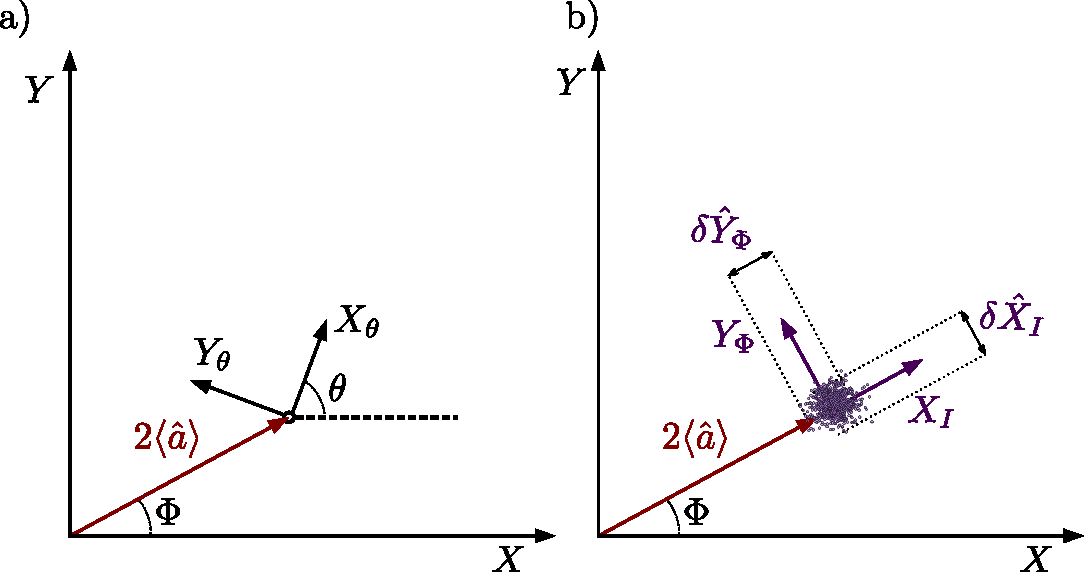
\includegraphics[width=0.8\textwidth]{chap_correlation/fig/fresnel.pdf}
    \caption{ \textbf{a)} Fresnel representation of a classical state. \textbf{b)} Quantum representation 
    of the quadrature operators. The spreaded cloud of points around the mean value $(\langle \hX \rangle, \langle \hY \rangle)$ represents several measurements of the same quantum state. The area of the cloud 
    is bounded from below by the Heisenberg uncertainty principle. The quadratures $\hX_{I}$ and $\hY_{\Phi}$ are the amplitude and phase quadratures respectively.}
    \label{fig:fresnel}
\end{figure}


\begin{equation}
    \label{eq:commut}
    [\hX,\hY] = 2i.
\end{equation}
Consequently, the quadrature operators are non-commuting variables and cannot be simultaneously measured with arbitrary precision. This is a direct consequence of the Heisenberg uncertainty principle stating that the product of the uncertainties in the two quadrature measurements is bounded from below by a constant value.
More precisely, the variances $\Delta X^2 = \langle \hX^2 \rangle - \langle \hX \rangle^2$ and $\Delta Y^2 = \langle \hY^2 \rangle - \langle \hY \rangle^2$ must satisfy the inequality :
\begin{equation}
    \label{eq:uncertainty}
    \Delta X^2 \Delta Y^2 \geq 1
\end{equation}
In contrast with the classical case, the vector $(\langle \hX \rangle, \langle \hY \rangle)$ representing the expectation values of the operators is associated with uncertainties whose area is bounded by the Heisenberg principle. 
The state most closely resembling a classical field is the one in which the fluctuations in both quadratures saturate \autoref{eq:uncertainty}. In this case, the uncertainty area assumes a circular shape with a diameter $E_0$ in the phase space, as illustrated in \autoref{fig:fresnel} \textbf{b)}. In this figure, the field and its fluctuations are not represented on the same scale; a laser field comprises a very large number of photons, whereas the fluctuations are of the order of the field of a single photon. 
Such a minimum uncertainty state is referred to as a coherent state while the corresponding fluctuations define the standard quantum fluctuations. Coherent
state are typically produced by a laser way above threshold and are the eigenvector of the annihilation operator $\hat{a}$.

\subsection{Intensity and phase fluctuations}

The choice of a given set of quadrature operators is arbitrary and corresponds to a choice of phase reference.
Moving to another set of operators $\hX_{\theta},\hY_{\theta}$ consists in a rotation in the phase space :

\begin{equation}
    \hX_{\theta} = \hX \cos(\theta) + \hY \sin(\theta) \ \ \mathrm{and} \ \
    \hY_{\theta} = -\hX \sin(\theta) + \hY \cos(\theta).
\end{equation}

The rotated operators satisfy the same commutation relation \ref{eq:commut} and the uncertainty relation \ref{eq:uncertainty} remains valid. 
However, a particular choice of quadratures is often made in the context of quantum optics \cite{grynberg_aspect_fabre} which consists in
chosing $\theta=\Phi$ where $\Phi$ is the phase of the mean field $\langle \hat{a}\rangle= |\hat{a}|e^{i\Phi}$.  The fluctuations of the corresponding quadrature
operators that we call $\hX_{I}$ and $\hY_{\Phi}$ are then proportionnal to intensity and phase fluctuations respectively as shown in \autoref{fig:fresnel} ~\textbf{b)}. In the case of 
a laser beam, the standard quantum limit is also referred to as the shot noise limit and ultimately originate from spontaneous emission of photons in the gain medium which yields a poissonian statistics in the photon arrival time \cite{grynberg_aspect_fabre}.
Indeed, the measurement of the intensity of a laser beam is subject to statistical noise scalling as the square root of the mean number of photons in the beam.

\begin{equation}
    \label{eq:shotnoise}
    \Delta \hat{N}^2 = \langle \hat{N}\rangle
\end{equation}
From an experimental point of view, this relation is helpfull since it provides a direct way to infer the standard quantum limit from an intensity measurement.   


\subsection{Squeezed states}
While vacuum fluctuations serve as a reference for quantum fluctuations, there is nevertheless no fundamental restriction against obtaining states in which the fluctuations of a given quadrature, $\hX_{\theta}$, are reduced below the standard quantum limit. Indeed, the Heisenberg inequality pertains to the product of uncertainties.
 This inequality remains satisfied provided that the fluctuations in the orthogonal quadrature $\hY_{\theta}$ increase accordingly. Graphically, their representation is obtained by squeezing the uncertainty area along the direction of the quadrature $\hX_{\theta}$ and stretching it along the direction of $\hY_{\theta}$. The resulting states are referred to as a squeezed state, and are of great interest 
 in quantum optics as they can be used to enhance the sensitivity of measurements. As an example, phase squeezed state are used in LIGO-VIRGO infrastrucutres to resolve the infinitesimal displacements of the interferometer mirrors induced by the passing gravitational waves.

\section{Photodectection}
\label{sec:photodetection}


A photodetector is a device that converts the energy of a photon into an electrical signal. The most common type of photodetector is the photodiode, which operates by generating a current in response to the absorption of photons. 
In principle, such devices allows to acquire and process all the information contained in the electromagnetic field by electronic means.
However, an optical field oscillates at hundreds of terahertz, which is far beyond the bandwidth of any electronic device. A photodiode can thus 
only provide a time-averaged signal, which is proportional to the intensity of the field. More precisely, the mean value of the photo-current $\bar{i}$ is proportionnal to the incoming photon flux as :

\begin{equation}
    \label{eq:photocurrent}
    \bar{i} = \eta e \dfrac{P}{\hbar\omega}
\end{equation}
where $\eta$ is the quantum efficiency of the photodetector, $e$ is the electron charge, $P$ is the power of the incoming light and $\hbar\omega$ is the energy of a single photon. 
In the ideal case $\eta=1$ where $100\%$ of the photons are converted into electrons the current statistics reproduce exactly the statistics of the incoming light.
However, in practice, the quantum efficiency is always less than one and the photodetector introduces losses that add to the photonic losses that the incoming beam may has already undergone.
Such losses are random events and subsequently lead any statistics to become Poissonian when they are large enough.


This being said, a incoming photon flux shot noise limited will produce a photocurrent that also follows a Poissonian statistics. For a mean number 
of electron $N_e$ produced by the photodetector, the variance is :

\begin{equation}
    \label{eq:n_e_variance}
    \Delta N_e^2 = N_e.
\end{equation}
From which we deduce the variance of the photocurrent on a time interval $\Delta t$ :
\begin{equation}
    \label{eq:photocurrent_variance}
    \Delta i^2 = \dfrac{e^2\Delta N_e^2}{\Delta t^2}=\dfrac{e^2N_e}{\Delta t^2}.
\end{equation}
Furthermore, by writting $N_e=\bar{i}\Delta t/e$ we obtain :
\begin{equation}
    \label{eq:photocurrent_variance2}
    \Delta i^2 = \dfrac{e\bar{i}}{\Delta t}.
\end{equation}
This relation shows that the variance of the photocurrent is inversely proportional to the time interval over which the current is measured. In the frequency
domain it means that the variance is proportionnal to the bandwidth of the measurement apparatus $\delta f=1/2\Delta t$. 
Furthermore, in the case where the latter can be modeled by a narrow band-pass filter centered on an analysis frequency $\omega_c$ it can be shown \cite{fabre_houches_97}
that the variance of the photocurrent is related to its power spectral density as :

\begin{equation}
    \label{eq:photocurrent_variance3}
    \Delta i^2 = 2\delta f S_i(\omega).
\end{equation}
This is precisely how a spectrum analyzer behaves. It measures the power spectral density of the photocurrent $S_i(\omega)$ by integrating the variance of the current over a given bandwidth $\delta f$ usually limited by the resolution 
bandwith (RBW) of the device.
At the end, we have a way to measure the power spectral density of the incoming light field by measuring the variance of the photocurrent. 
Let us now see how such a device can be used to measure the correlations between two fields.

\section{Balanced detection}

Intensity balanced detection is a common detection scheme used to suppress the classical noise commonly present in optical measurements.
The basic principle of this technique is to use two photodetectors, each measuring the intensity of an optical field, and to subtract their output photo-currents. If the two 
beams share the same classical noise, the subtraction will cancel it out, leaving only the quantum correlations. A representation of the balanced detection scheme is shown in \autoref{fig:balanced_detection}.
Usually, these kind of apparatus are also able to measure the sum of the two photo-currents which is proportional to the total noise of the two beams. However,
as we will see in the next section, measuring the difference together with the individual photo-currents is sufficient to obtain the correlation function of the two fields.
\begin{figure}
    \centering
    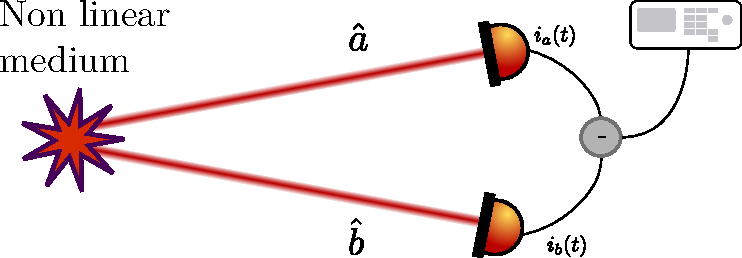
\includegraphics[width=0.8\textwidth]{chap_correlation/fig/balanced_detection.pdf}
    \caption{Balanced detection scheme. Example of a typical non linear medium producing two modes of the electromagnetic field $\hat{a}$ and $\hat{b}$. Each of them is sent to a photodiode that produces a photo-current carrying the noise
    of the beams. The output photo-currents are then subtracted to cancel the classical noise and sent into a spectrum analyzer.}
    \label{fig:balanced_detection}
\end{figure} 

\subsection{Difference measurement}
Let us consider two fields $\hat{a}$ and $\hat{b}$ impinging on two photodetectors as shown in \autoref{fig:balanced_detection}. Their respective intensity 
are given by their number operator $\hat{N}_a=\hat{a}^\dagger\hat{a}$ and $\hat{N}_b=\hat{b}^\dagger\hat{b}$.
We are interested in the intensity difference operator $\hat{N}_-$ defined as :
\begin{equation}
    \label{eq:diff_op}
    \hat{N_-} = \hat{a}^\dagger\hat{a} - \hat{b}^\dagger\hat{b}.
\end{equation}

As explained above, it is convenient to linearize each operator around its mean value :
\begin{equation}
    \begin{aligned}
    \hat{a} &= |\alpha|e^{i\Phi} + \delta \hat{a} \\
    \hat{b} &= |\beta|e^{i\Psi} + \delta \hat{b}
    \end{aligned}
\end{equation}
where $|\alpha|e^{i\Phi}$ and $|\beta|e^{i\Psi}$ are the mean values of the two fields and $\delta \hat{a}$ and $\delta \hat{b}$ are their respective fluctuations.
The difference operator can then be expressed to first order in the fluctuations as :
\begin{equation}
    \label{eq:diff_op2}
    \begin{aligned}
    \hat{N_-} &= (|\alpha|^2e^{i\Phi}+\delta \hat{a}^\dagger)(|\alpha|e^{i\Phi}+\delta \hat{a}) - (|\beta|^2e^{i\Psi}+\delta \hat{b}^\dagger)(|\beta|e^{i\Psi}+\delta \hat{b}) \\
    &= |\alpha|^2 - |\beta|^2 +(|\alpha|\delta \hX_a^\Phi + |\beta|\delta \hX_b^\Psi) 
    \end{aligned}
\end{equation}



\section{Correlations in continuous-variables quantum optics}
\label{sec:corr_cv}
As a very general statement, two quantities are said to be correlated if they ultimately originate from the same source or quantum process. In this case, a knowledge of one of the two quantities gives informations about the other.
Take the example of a two photons emission by a non linear process such as a Type II spontaneous parametric down conversion (SPDC). Their correlations is of several natures. The first and most obvious one is temporal in the sense that the two photons are emitted at the same time. This can be
quantified by looking at the second order intensity correlation function $g^{(2)}(t,t')$, which is the probability of detecting a photon at time $t$ and another one at time $t'$ \cite{hanbury_brown_twiss_1956}. They can also 
be correlated through their polarization meaning that if one photon is detected in a given polarization, the other one will be detected in the orthogonal polarization. Reversing the picture,
the measurement of a given type of correlations can thus provide informations about the quantum nature of the process that generated them.

The question of correlations can also be asked for a field and a version of itself that is delayed in time or shifted in space. In this case, one is in fact looking at the coherence of the field. 
To keep a general descrption let us consider a quantum operator evolving in time $\hat{f}(t)$. The autocorrelation of $\hf$ at time $t$ and $t'$ is defined as :

\begin{equation}
    \label{eq:autocorr}
    C_{\hf}(t,t') = \langle \hf(t)\hf(t') \rangle = \langle \delta \hf(t) \delta \hf(t') \rangle
\end{equation}
where $\delta \hf(t) = \hf(t) - \langle \hf(t) \rangle$ is the fluctuation of the operator around its expectation value. If the process at stake 
is stationary, $\langle \hf(t) \rangle$ does not depend on $t$ and the correlation function depends only on the time difference $\tau= t-t'$ \cite{bachor_guide_1998}. In this case,
the Wiener-Khinchin theorem states that the autocorrelation function is related to the spectral density of the field $\mathcal{S}_{\hf}(\omega)$ by a Fourier transform \cite{fabre_houches_97} :

\begin{equation}
    \label{eq:autocorr_spectral}
    S_{\hf}(\omega) = \int_{-\infty}^{+\infty} C_{\hf}(\tau) e^{-i\omega \tau} d\tau.
\end{equation}

In the same manner it is possible to define the cross-correlation between two operators $\hf_1$ and $\hf_2$ as :

\begin{equation}
    \label{eq:crosscorr}
    C_{\hf_1,\hf_2}(t,t') = \langle \hf_1(t)\hf_2(t') \rangle = \langle \delta \hf_1(t) \delta \hf_2(t') \rangle
\end{equation}

\section{Experimental implementation}
\label{sec:exp_impl}


\subsection{Excitation scheme}

The set up used is similar to the one used in the previous experiemnt with the addition of a balanced detection scheme that will be detailled in the next section. 
The microcavity is the same as the one used in the previous chapters but the experiment is runned at the working point B10-C10 (see ?????).

We create a static polariton fluid by shinning a pump laser beam of diameter $w=\SI{100}{\micro\meter}$ at normal incidence on the microcavity. The laser is detuned from the polariton resonance by
$\delta = \SI{35}{\giga\hertz}$ in order operate in a bistable regime. A typical real space image of the polariton fluid is shown in \autoref{fig:real_space} \textbf{a)}. 
 
\begin{figure}
    \centering
    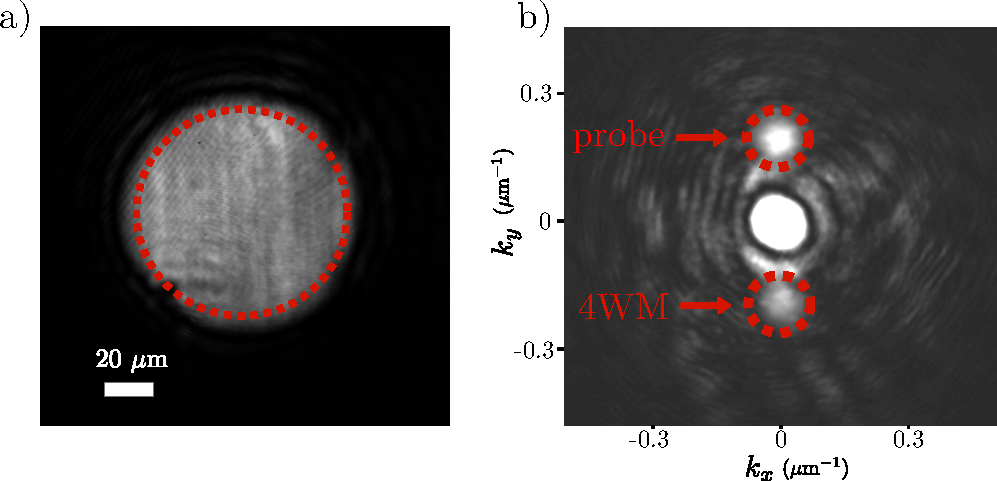
\includegraphics[width=0.8\textwidth]{chap_correlation/fig/r_and_k_space.pdf}
    \caption{\textbf{a)} Real space image of a polariton fluid operating on the high density branch of the bistability loop. The image is taken at the working point B10-C10. The red dashed circle represents
    the pinhole applied to the image to filter out the signal coming from the edges of the fluid. \textbf{b)} Corresponding k-space image of the polariton fluid when a weak probe is exciting the normal branch at $k_{pr}=\SI{0.2}{\per\micro\meter}$. 
    The direct transmission of the probe is pointed out by the red arrow on top of the image while its four wave mixing signal is visible at $-k_{pr}$. The red dasehd circles represent the pinholes applied 
    to the image to isolate each signal before sending it to the balanced detection scheme. }
    \label{fig:real_space}
\end{figure}
\subsection{Experimental setup}
The set up used is similar to the one used in the previous chapter with the addition of a balanced detection scheme. The latter is detailed in 
\autoref{fig:setup}. First an intermadiate plane 